% =====================================================================
%  Σχεδιασμός Ενσωματωμένων Συστημάτων -- 1η Εργαστηριακή Άσκηση
%  Ομάδα 40
%
%  ΜΕΤΑΓΛΩΤΤΙΣΗ: XeLaTeX (στο Overleaf: Menu -> Compiler -> XeLaTeX).
%  Το αρχείο latexmkrc του project επιβάλλει ήδη XeLaTeX.
% =====================================================================
\documentclass[11pt,a4paper]{article}

% ---------- Γραμματοσειρές / γλώσσα ----------
\usepackage{fontspec}
\setmainfont{LibertinusSerif}[
  Extension=.otf, UprightFont=*-Regular, BoldFont=*-Bold,
  ItalicFont=*-Italic, BoldItalicFont=*-BoldItalic]
\setsansfont{LibertinusSans}[
  Extension=.otf, UprightFont=*-Regular, BoldFont=*-Bold, ItalicFont=*-Italic]
\setmonofont{DejaVuSansMono}[
  Extension=.ttf, UprightFont=*, BoldFont=*-Bold, Scale=0.85]
\usepackage[english,greek]{babel}

% ---------- Διάταξη ----------
\usepackage[margin=2.3cm]{geometry}
\usepackage[table]{xcolor}
\usepackage{graphicx}
\usepackage{booktabs,tabularx,multirow,array}
\usepackage{float}
\usepackage{caption,subcaption}
\usepackage{enumitem}
\usepackage{amsmath,amssymb}
\usepackage{siunitx}
\usepackage{listings}
\usepackage[most]{tcolorbox}
\usepackage{pgfplots}
\pgfplotsset{compat=1.18}
\usepackage{fancyhdr}
\usepackage[hidelinks]{hyperref}

\sisetup{group-minimum-digits=4, group-separator={\,}}
\captionsetup{font=small, labelfont=bf}
\setlist{itemsep=2pt, topsep=4pt}
\renewcommand{\arraystretch}{1.15}

\definecolor{accent}{HTML}{1F4E79}
\definecolor{codebg}{HTML}{F5F7FA}
\definecolor{good}{HTML}{2E7D32}
\definecolor{bad}{HTML}{C62828}

\lstset{
  language=C, basicstyle=\ttfamily\small, backgroundcolor=\color{codebg},
  keywordstyle=\color{accent}\bfseries, commentstyle=\color{gray}\itshape,
  stringstyle=\color{good}, frame=single, rulecolor=\color{gray!40},
  breaklines=true, columns=fullflexible, keepspaces=true,
  showstringspaces=false, xleftmargin=4pt, xrightmargin=4pt,
  morekeywords={uint32_t,uint64_t,uint8_t,register}
}

% Πλαίσιο για σύντομες "έξυπνες" παρατηρήσεις
\newtcolorbox{insight}[1][Παρατήρηση]{
  enhanced, breakable, colback=accent!4, colframe=accent!70,
  fonttitle=\bfseries\small, title=#1, boxrule=0.6pt, arc=2pt,
  left=6pt, right=6pt, top=4pt, bottom=4pt}

\newcommand{\TODO}[1]{\textcolor{bad}{\textbf{[#1]}}}
\newcommand{\code}[1]{\texttt{#1}}
\newcommand{\en}[1]{\foreignlanguage{english}{#1}}

\setlength{\headheight}{14pt}
\pagestyle{fancy}
\fancyhf{}
\fancyhead[L]{\small Σχεδιασμός Ενσωματωμένων Συστημάτων}
\fancyhead[R]{\small 1η Εργαστηριακή Άσκηση -- Ομάδα 40}
\fancyfoot[C]{\thepage}

% =====================================================================
\begin{document}

\begin{titlepage}
  \centering
  {\large ΕΘΝΙΚΟ ΜΕΤΣΟΒΙΟ ΠΟΛΥΤΕΧΝΕΙΟ\par}
  {\normalsize Σχολή Ηλεκτρολόγων Μηχανικών και Μηχανικών Υπολογιστών\par}
  {\normalsize Εργαστήριο Μικροϋπολογιστών και Ψηφιακών Συστημάτων\par}
  \vspace{3cm}
  {\Large Σχεδιασμός Ενσωματωμένων Συστημάτων\par}
  \vspace{0.4cm}
  {\normalsize 9ο Εξάμηνο ΗΜΜΥ\par}
  \vspace{1.5cm}
  {\color{accent}\rule{0.8\textwidth}{0.8pt}\par}
  \vspace{0.4cm}
  {\huge\bfseries 1η Εργαστηριακή Άσκηση\par}
  \vspace{0.3cm}
  {\Large Βελτιστοποίηση αλγορίθμων για χαμηλή κατανάλωση\\ ενέργειας και υψηλή απόδοση\par}
  \vspace{0.4cm}
  {\color{accent}\rule{0.8\textwidth}{0.8pt}\par}
  \vfill
  {\large\bfseries Ομάδα 40\par}
  \vspace{0.4cm}
  \begin{tabular}{ll}
    Μιχαήλ Παναγόπουλος & ΑΜ: 03122061 \\
    Αθανάσιος Φειδάκης  & ΑΜ: 03122676 \\
  \end{tabular}
  \vspace{2cm}
\end{titlepage}

\tableofcontents
\newpage

% =====================================================================
\section{Ζητούμενο 1ο}
% =====================================================================

% ---------------------------------------------------------------------
\subsection{Ερώτημα 1}
% ---------------------------------------------------------------------

Έπειτα από μελέτη του datasheet της πλακέτα τα ζητούμενα χαρακτηριστικά συνοψίζονται στον Πίνακα~\ref{tab:board}.

\begin{table}[H]
\centering
\caption{Βασικά χαρακτηριστικά του μικροελεγκτή Renesas Synergy S7G2.}
\label{tab:board}
\begin{tabularx}{\textwidth}{@{}l X@{}}
\toprule
\textbf{Χαρακτηριστικό} & \textbf{Τιμή} \\
\midrule
Πυρήνας & \en{Arm Cortex-M4F} (FPU απλής ακρίβειας, εντολές DSP/SIMD, MPU) \\
Μέγιστη συχνότητα & \SI{240}{MHz} (με αυτήν τρέχει το πρόγραμμα)\\
Μνήμη \en{Code Flash} & έως \SI{4}{MB} (σε άλλη έκδοση ίσως \SI{3}{MB} \\
Μνήμη \en{Data Flash} & \SI{64}{KB} \\
Μνήμη SRAM & \SI{640}{KB} on-chip SRAM \\
Κρυφές μνήμες & Ο \en{Cortex-M4} \textbf{δεν} διαθέτει \en{L1 instruction/data cache}.
  Η μόνη κρυφή μνήμη είναι η \textbf{\en{Flash Cache (FCACHE)}}, η οποία βρίσκεται μπροστά από την
  \en{code flash} και κρύβει τους κύκλους αναμονής της flash σε υψηλές
  συχνότητες. Η SRAM προσπελαύνεται απευθείας, χωρίς \en{cache}. \\
\bottomrule
\end{tabularx}
\end{table}

% ---------------------------------------------------------------------
\subsection{Ερώτημα 2}
% ---------------------------------------------------------------------

\subsubsection*{Αλλαγές στον κώδικα}

Οι μόνες αλλαγές
έγιναν στο \code{hal\_entry}, στο οποίο η συνάρτηση \code{phods\_motion\_estimation} καλείται 10 φορές και κάθε κλήση ``περικλείεται'' από δύο
αναγνώσεις του \code{DWT->CYCCNT}. Υπολογίζονται με προσοχή για πιθανές υπερχειλίσεις και λάθος μετατροπές τύπων δεδομένων τα στατιστικά min/max/mean και διαβάζονται από το \en{Variables} του \en{debugger}, με \en{breakpoint} στο τελικό
\code{while(1)}. 

\subsubsection*{Αποτελέσματα}

\begin{table}[H]
\centering
\caption{Χρόνος εκτέλεσης του αρχικού κώδικα (10 εκτελέσεις, $N=M=10$, $B=5$).}
\label{tab:base}
\begin{tabular}{@{}lrr@{}}
\toprule
 & \textbf{Κύκλοι} & \textbf{Χρόνος (ms)} \\
\midrule
Ελάχιστος  & \num{445306}   & \num{1.855442} \\
Μέγιστος   & \num{445308}   & \num{1.855450} \\
Μέσος όρος & \num{445306.2} & \num{1.855443} \\
\bottomrule
\end{tabular}
\end{table}

\subsubsection*{Σχόλια - Παρατηρήσεις}
Προκειμένου να δούμε αναλυτικά τους χρόνους εκτέλεσης των 10 επαναλήψεων κρατάμε ιστορικό σε πίνακα (\code{cycles[10]}). Η διαφορά μεγίστου ελαχίστου είναι μόλις 2 κύκλοι. Ο χρόνος εκτέλεσης είναι πρακτικά ίδιος, σχεδόν ντετερμινιστικός. Αυτό μπορεί να εξηγηθεί από την απουσία των παρεμβάσεων του λειτουργικού, από το
in-order pipeline του επεξεργαστή και την απουσία data cache με μεταβλητή συμπεριφορά. Ούτε η πρώτη
εκτέλεση είναι πιο αργή, όπως θα περιμέναμε λόγω κρύας FCACHE.


\noindent Το αντίστοιχο \en{screenshot} του \en{debugger} βρίσκεται στο Παράρτημα~\ref{app:z1}
(Σχήμα~\ref{fig:app_q2}).

% ---------------------------------------------------------------------
\subsection{Ερώτημα 3}
% ---------------------------------------------------------------------

Κάθε έκδοση \code{solution1b\_vX.c} προσθέτει λίγες επιπλέον ιδέες για την βελτίωση του κώδικα πάνω στην προηγούμενη έκδοση. Έτσι
η διαφορά κύκλων μεταξύ διαδοχικών εκδόσεων μετρά τη συνεισφορά του κάθε μετασχηματισμού
χωριστά. Ο συμβολισμός $\Delta$ δείχνει τη μεταβολή
σε σχέση με την \emph{προηγούμενη} έκδοση και το \en{speedup} τη βελτίωση σε σχέση με τον \emph{αρχικό} κώδικα.

% ---- helper για τον πίνακα αποτελεσμάτων κάθε έκδοσης
\newcommand{\vres}[7]{%
\begin{center}\small
\begin{tabular}{@{}rrrrrr@{}}
\toprule
\textbf{Μέσος (κύκλοι)} & \textbf{Min} & \textbf{Max} & \textbf{Μέσος (ms)} & \textbf{$\Delta$ vs προηγ.} & \textbf{Speedup} \\
\midrule
\num{#1} & \num{#2} & \num{#3} & \num{#4} & #5 & #6$\times$ \\
\bottomrule
\end{tabular}\\[2pt]
{\footnotesize #7}
\end{center}}

% ---------------- v1
\subsubsection{v1 - Αρχικοποίηση διανυσμάτων μέσα στον κύριο βρόχο \en{Loop merge}}
\textbf{Ιδέα:} ο ξεχωριστός διπλός βρόχος που μηδενίζει τα \code{vectors\_x/y} συγχωνεύεται
με τον βρόχο που διατρέχει τα μπλοκ, αφού οι δείκτες των δύο αυτών loops τρέχουν στο ίδιο space.\\
\vres{442432.6}{442432}{442438}{1.843469}{\textcolor{good}{$-0.65\%$}}{1.007}{}
\textbf{Σχόλιο:} Με την αλλαγή αυτή αποφεύγεται το overhead του βρόχου αρχικοποίησης των διανυσμάτων. Η βελτίωση είναι αρκετά μικρή. Αυτό εξηγείται καθώς γλιτώνουμε μόνο το \en{overhead} ενός βρόχου πάνω σε
$(N/B)^2=4$ στοιχεία.

% ---------------- v2
\subsubsection{v2 - Κοινός βρόχος για την αναζήτηση σε $x$ και $y$ (\en{Loop merge})}
\textbf{Ιδέα:} οι δύο βρόχοι \code{for(i=-S; i<S+1; i+=S)} για τους άξονες $x$ και $y$ έχουν
ίδια όρια, οπότε συγχωνεύονται σε έναν. Μέσα στον ίδιο διπλό βρόχο $k,l$, πλέον, υπολογίζονται ταυτόχρονα τα \code{distx} και
\code{disty}. Το \code{current} διαβάζεται μία φορά και χρησιμοποιείται και για τα δύο.\\
\vres{394590.4}{394590}{394594}{1.644127}{\textcolor{good}{$-10.81\%$}}{1.129}{}
\textbf{Σχόλιο:} Με την αλλαγή αυτή επιτυγχάνουμε το μισό \en{overhead} των βρόχων με δείκτες $i,k,l$ και τις μισές αναγνώσεις του
\code{current} από τη flash. Ωστόσο κάθε επανάληψη κάνει πλέον διπλή δουλειά.

% ---------------- v3
\subsubsection{v3 -- \en{Loop unrolling} του \code{while(S>0)}}
\textbf{Ιδέα:} ο βρόχος του $S$ εκτελείται πάντα ακριβώς 3 φορές ($S=4,2,1$), άρα ξεδιπλώνεται πλήρως. Tο σώμα του loop γίνεται \en{macro} \code{s\_loop(S)} και καλείται ως
\code{s\_loop(4); s\_loop(2); s\_loop(1);}. Αποφεύγουμε την λύση της συνάρτησης η οποία θα εισήγαγε επιπλέον καθυστερήσεις υπολογισμών διευθύνσεων, εντολών jump προς αυτές και αποθήκευσης δεδομένων στην stack. Μαζί με τον βρόχο φεύγει και η διαίρεση \code{S=S/2}.\\
\vres{394143}{394143}{394143}{1.642263}{\textcolor{good}{$-0.11\%$}}{1.130}{}
\textbf{Σχόλιο:} Παρατηρούμε ελάχιστο όφελος. Αυτό οφείλεται στο γεγονός ότι ο βρόχος που αφαιρέθηκε είναι εξωτερικός (12 επαναλήψεις συνολικά),
άρα το overhead του είναι αμελητέο. Κερδίσαμε $\approx\num{450}$ κύκλους, δηλαδή $\approx 37$ κύκλους ανά επανάληψη που
αφαιρέθηκε (σύγκριση, \en{branch}, διαίρεση του $S$). Ο μεγαλύτερος κώδικας που προκύπτει δεν φαίνεται να έχει επίπτωση στην FCACHE.

% ---------------- v4
\subsubsection{v4 - \en{Loop unrolling} του βρόχου των υποψηφίων $i$}
\textbf{Ιδέα:} ο βρόχος \code{for(i=-S; i<S+1; i+=S)} εκτελείται πάντα 3 φορές ($-S,0,+S$), επομένως τον
ξεδιπλώνουμε με το i πλέον αν είναι σταθερό κατά το compile. Προστίθεται νέα \en{macro} \code{i\_loop(i)} που καλέίται από την \code{s\_loop(S)} 3 φορές
\code{i\_loop(-S); i\_loop(0); i\_loop(S);}.\\
\textbf{Αναμενόμενο:} αφαιρείται το \en{overhead} 36 βρόχων. Επιπλέον, επειδή το $i$ είναι πλέον σταθερά του compile, οι έλεγχοι ορίων
δεν φορτώνουν το $i$ από το stack σε κάθε \en{pixel}.
\vres{377535.4}{377535}{377539}{1.573064}{\textcolor{good}{$-4.21\%$}}{1.180}{}
\textbf{Σχόλιο:} Με αυτήν την αλλαγή αφαιρείται το \en{overhead} 36 βρόχων. Επιπλέον το $i$ δεν είναι μεταβλητή αλλά σταθερά κατά το compile, επομένως δεν υφίσταντα προσβάσεις στην μνήμη για αυτή την μεταβλητή. Το μεγαλύτερο κομμάτι από το χρονικό όφελος πρέπει να αποδοθεί στην αλλαγή του "τύπου" του $i$ και όχι στο \en{overhead} των λίγων 
βρόχων από τους οποίους απαλλασσόμαστε. Αξίζει να σημειωθεί ότι αντίστοιχο όφελος είχαμε και στο προηγούμενο version με το $S$, ωστόσο το $i$ χρησιμοποιείται πολύ περισσότερες φορές στο εσωτερικό loop για bounary check στο previous frame.

% ---------------- v5
\subsubsection{v5 - Αποφυγή περιττών επαναυπολογισμών μέσα στο \en{loop} του \en{block}}
\textbf{Ιδέα:} τα \code{vectors\_x[x][y]}, \code{vectors\_y[x][y]}, \code{B*x}, \code{B*y} είναι
αμετάβλητα μέσα στους βρόχους των \en{pixels}, αλλά υπολογίζονται και φορτώνονται από
τη μνήμη σε \emph{κάθε} εμφάνισή τους (υπολογισμοί δεικτών για τις 2 διαστάσεις των πινάκων, φορτώσεις
δεικτών και μεταβλητών). Ορίζουμε επομένως, τοπικές μεταβλητές \code{vx, vy}, αντίγραφα των διανυσμάτων, τα οποία γράφονται στους
πίνακες \code{vectors\_x[x][y]} μία φορά στο τέλος της επεξεργασίας του block, και \code{bx=B*x, by=B*y} τα οποία υπολογίζονται μία φορά ανά block).\\
\vres{222121.5}{222121}{222126}{0.925506}{\textcolor{good}{$-41.17\%$}}{2.005}{}
\textbf{Σχόλιο:} Με την λύση αυτή προκύπτει πολύ μεγάλο όφελος αφού σε κάθε εσωτερική επανάληψη υπάρχουν 16 προσπελάσεις στα
\code{vectors\_*} και πολλοί πολλαπλασιασμοί \code{B*x}/\code{B*y}. Παρατηρούμε μείωση κατά $\approx\num{155400}$ κύκλους. Αυτό αποδεικνύει πόσο ακριβός είναι ο επαναλαμβανόμενος υπολογισμός διευθύνσεων πινάκων πολλών διαστάσεων.

% ---------------- v6
\subsubsection{v6 -- Κοινός κεντρικός υποψήφιος και φθηνότερη υλοποίηση της συνάρτησης \code{abs}}
\textbf{Ιδέα:} για $i=0$ ο υποψήφιος στον άξονα $x$ και στον άξονα $y$ είναι το ίδιο μπλοκ, άρα η απόστασή του υπολογίζεται μία φορά και χρησιμοποιείται και στις δύο
συγκρίσεις. Προσθέτουμε νέα \en{macro} \code{c\_loop} στη θέση του \code{i\_loop(0)}. Επιπλέον, η απόλυτη διαφορά υπολογίζεται με μία αφαίρεση.
Το \code{if(p1-p2>0) ... else ...} γίνεται \code{d = p1-p2; dist += (d<0) ? -d : d;}.\\
\vres{184796.5}{184796}{184801}{0.769985}{\textcolor{good}{$-16.80\%$}}{2.410}{}
\textbf{Σχόλιο:} Πλέον, ανά βήμα υπολογίζονται 5 αποστάσεις block αντί για 6, δηλαδή $\approx 1/6$ λιγότερη
δουλειά στον εσωτερικό βρόχο, με επιπλέον όφελος από την αποδοτικότερη υλοποίηση της συνάρτησης abs. Η μέτρηση ($-16.80\%$) συμπίπτει σχεδόν με την πρόβλεψη ($-16.7\%$). Ο
χρόνος, λοιπόν, είναι πρακτικά ανάλογος του πλήθους των υπολογισμών αποστάσεων ανάμεσα σε blocks. Το \code{abs} με μία
αφαίρεση έχει αμελητέα επίδραση. Αυτό είναι λογικό, αφού και η αρχική μορφή εκτελεί απλά μία επιπλέον αφαίρεση μετά τον έλεγχο της συνθήκης.

% ---------------- v7
\subsubsection{v7 - Αντιγραφή σε SRAM και \en{zero padding} του προηγούμενου frame}
\textbf{Ιδέα:} τα \code{current}/\code{previous} είναι \code{const}, άρα βρίσκονται στην
αργή flash, ενώ οι μη-\code{const} πίνακες βρίσκονται στη SRAM. Επιπλέον οι 8 συγκρίσεις ορίων ανά
\en{pixel} υπάρχουν μόνο για να επιστρέφουν 0 έξω από το \en{frame}. Αν το \en{frame} περιβληθεί από
μηδενικά, οι συγκρίσεις αυτές γίνονται περιττές. Ορίζουμε τον πίνακα \code{static int prev\_pad[N+2p][M+2p]} στην SRAM. Σε κάθε κλήση αντιγράφεται εκεί το \code{previous}, με zero padding περιμετρικά και το τρέχον block αντιγράφεται
στο τοπικό \code{cb[Bx][By]}. Ο εσωτερικός βρόχος γίνεται απλώς
\code{p2 = prev\_pad[bx+vx+i+k+p][by+vy+l+p]}, χωρίς κανέναν έλεγχο.\\
\textbf{Αναμενόμενο:} απαλλασόμαστε από όλες τις διακλαδώσεις ελέγχου και οι αναγνώσεις πλέον
γίνονται από SRAM. Το κόστος της αντιγραφής ($\num{100}+4\cdot 25$ στοιχεία) είναι μικρό.
\vres{119072.8}{119071}{119073}{0.496137}{\textcolor{good}{$-35.57\%$}}{3.740}{}
\textbf{Σχόλιο:} Παρατηρούμε μεγάλη μείωση καθώς απαλλασόμαστε από όλες τις διακλαδώσεις ελέγχου και οι αναγνώσεις πλέον
γίνονται από την SRAM και όχι από την αργή FLACHE. Το κόστος της αντιγραφής ($\num{100}+4\cdot 25$ στοιχεία) και το επιπλέον memory footprint $(10+14)^2\cdot\SI{4}{B}=\SI{2.3}{KB}$ είναι σχετικά μικρά. Το περιθώριο $p=7$ είναι \emph{ακριβώς} το απαραίτητο, αφού η μέγιστη συνολική
μετατόπιση είναι $4+2+1=7$.

\begin{insight}[Σχετικά με το \en{hint} της εκφώνησης]
Βελτιστοποιήσεις που ``αντιγράφουν'' ή αναδιατάσσουν δεδομένα έχουν όφελος μόνο αν τα δεδομένα
μετακομίσουν σε ταχύτερη μνήμη. Αν δηλώναμε π.χ.\ τον \code{prev\_pad} ως \code{const} (προϋπολογισμένο
στη flash), θα γλιτώναμε τους ελέγχους ορίων, αλλά οι αναγνώσεις θα συνέχιζαν να πληρώνουν τους
\en{wait states} της flash. Αντίστροφα, ό,τι δεν είναι \code{const} ζει στη SRAM και η πρόσβαση σε
αυτό είναι ήδη γρήγορη. Με τις τρέχουσες μετρήσεις δεν μπορούμε να διαχωρίσουμε πόσο από το $-35.6\%$
οφείλεται στη SRAM και πόσο στην αφαίρεση των ελέγχων. Ένα πείραμα με \code{const} πίνακα
\en{padding} στη flash θα το ξεχώριζε.
\end{insight}

% ---------------- v8
\subsubsection{v8 -- Δείκτες γραμμής και \code{register} μεταβλητές}
\textbf{Ιδέα:} στον εσωτερικό βρόχο ($l$) διατρέχουμε μόνο ως προς την στήλη των πινάκων. Υπολογίζουμε επομένως την διεύθυνση της γραμμής μία φορά ανά $k$ και την αποθηκεύουμε σε δείκτη. Επίσης γνωρίζουμε ότι στο \code{-O0} ο \code{gcc} κρατά όλες τις μεταβλητές στη στοίβα, εκτός από όσες
δηλώνονται \code{register}. Για αυτόν τον λόγο επιλέγουμε χειροκίνητα τις πιο συχνά χρησιμοποιούμενες μεταβλητές (\code{cr}, \code{pr},
\code{qr}, \code{k, l, d, p1, distx, disty, distc}) να δηλώνονται ως register, ώστε η πρόσβαση σε αυτές να είναι πολύ πιο γρήγορη.

\vres{49504}{49504}{49504}{0.206267}{\textcolor{good}{$-58.43\%$}}{8.995}{}
\textbf{Σχόλιο:} Παρατηρούμε την μεγαλύτερη σχετική βελτίωση. Το πολύ μεγάλο όφελος έρχεται εξαιτίας της μετάβασης από υπολογισμούς
διεύθυνσης και \en{load/store} στη στοίβα σε μία φόρτωση με \en{offset} από \en{register}.

% ---------------- v9
\subsubsection{v9 -- SIMD SAD με την εντολή DSP \code{USADA8}}
\textbf{Ιδέα:} η \code{USADA8(a,b,acc)} του \en{Cortex-M4} υπολογίζει
$acc+\sum_{j=0}^{3}|a_j-b_j|$ για 4 \en{unsigned bytes} σε έναν κύκλο, δηλαδή ακριβώς τον πυρήνα του SAD.\\
\textbf{Αλλαγές:}
\begin{itemize}[leftmargin=*]
  \item Τα \code{cb} και \code{prev\_pad} γίνονται \code{uint8\_t}, ώστε 4 γειτονικά \en{pixels} να
  φορτώνονται με ένα \en{32-bit load} (ο \en{Cortex-M4} επιτρέπει \en{unaligned} φορτώσεις). Αυτό γίνεται
  μέσω \en{packed struct}, με την ίδια τεχνική που χρησιμοποιεί το CMSIS.
  \item Τα \en{pixels} του \code{images.h} είναι \en{signed} ($-128\ldots124$). Κατά την αντιγραφή
  προστίθεται \code{BIAS=128}. Επειδή $|(a+128)-(b+128)|=|a-b|$, τα SAD και τα διανύσματα μένουν
  \emph{ακριβώς} ίδια. Το \en{padding} γεμίζει με \code{0+BIAS}.
  \item Οι στήλες επεξεργάζονται ανά 4 και οι υπόλοιπες \code{By\%4} με τον βαθμωτό κώδικα, οπότε ο κώδικας
  δουλεύει για κάθε $B_x,B_y$.
\end{itemize}
\textbf{Αναμενόμενο:} για $B=5$, κάθε γραμμή μπλοκ θέλει 1 \code{USADA8} + 1 βαθμωτό \en{pixel}
αντί για 5 βαθμωτά. Επιπλέον, οι πίνακες γίνονται $4\times$ μικρότεροι.
\vres{37085.8}{37084}{37086}{0.154524}{\textcolor{good}{$-25.08\%$}}{12.008}{}
\textbf{Σχόλιο:} το όφελος είναι μικρότερο από το θεωρητικό $\sim$$3\times$ στον εσωτερικό βρόχο, για δύο
λόγους. Πρώτον, με $B=5$ μόνο τα $4/5$ των \en{pixels} περνούν από SIMD. Δεύτερον, στο \code{-O0} η
\code{LOAD4} και η κλήση του \en{intrinsic} κοστίζουν επιπλέον εντολές. Για $B_y$ πολλαπλάσιο του 4
(π.χ.\ 4, 8, 16) το κέρδος θα ήταν σαφώς μεγαλύτερο. Εδώ εμφανίζεται και μια ευθεία
σχέση ανάμεσα στο μέγεθος μπλοκ και το \en{hardware}: πλάτος SIMD = 4 \en{bytes} = εύρος του \en{bus}.



% ---------------- Summary
\subsubsection*{Συγκεντρωτικά αποτελέσματα}

\begin{table}[H]
\centering
\caption{Συγκεντρωτικός πίνακας όλων των εκδόσεων.}
\label{tab:summary}
\small
\begin{tabular}{@{}llrrrr@{}}
\toprule
\textbf{Έκδ.} & \textbf{Μετασχηματισμός} & \textbf{Μέσος (κύκλοι)} & \textbf{Χρόνος (ms)} & \textbf{$\Delta$ vs προηγ.} & \textbf{Speedup} \\
\midrule
Αρχικός & -- & \num{445306.2} & \num{1.855443} & -- & 1.00$\times$ \\
v1 & Συγχώνευση αρχικοποίησης & \num{442432.6} & \num{1.843469} & $-0.65\%$ & 1.01$\times$ \\
v2 & Συγχώνευση βρόχων $x$/$y$ & \num{394590.4} & \num{1.644127} & $-10.81\%$ & 1.13$\times$ \\
v3 & \en{Unroll} βρόχου $S$ & \num{394143.0} & \num{1.642263} & $-0.11\%$ & 1.13$\times$ \\
v4 & \en{Unroll} βρόχου $i$ & \num{377535.4} & \num{1.573064} & $-4.21\%$ & 1.18$\times$ \\
v5 & \en{Scalar replacement} / \en{LICM} & \num{222121.5} & \num{0.925506} & $-41.17\%$ & 2.00$\times$ \\
v6 & Κοινός κεντρικός υποψ. + \code{abs} & \num{184796.5} & \num{0.769985} & $-16.80\%$ & 2.41$\times$ \\
v7 & SRAM + \en{zero padding} & \num{119072.8} & \num{0.496137} & $-35.57\%$ & 3.74$\times$ \\
v8 & Δείκτες γραμμής + \code{register} & \num{49504.0} & \num{0.206267} & $-58.43\%$ & \textbf{9.00$\times$} \\
v9 & SIMD \code{USADA8} & \num{37085.8} & \num{0.154524} & $-25.08\%$ & \textbf{12.01$\times$} \\
\bottomrule
\end{tabular}
\end{table}

\begin{figure}[H]
\centering
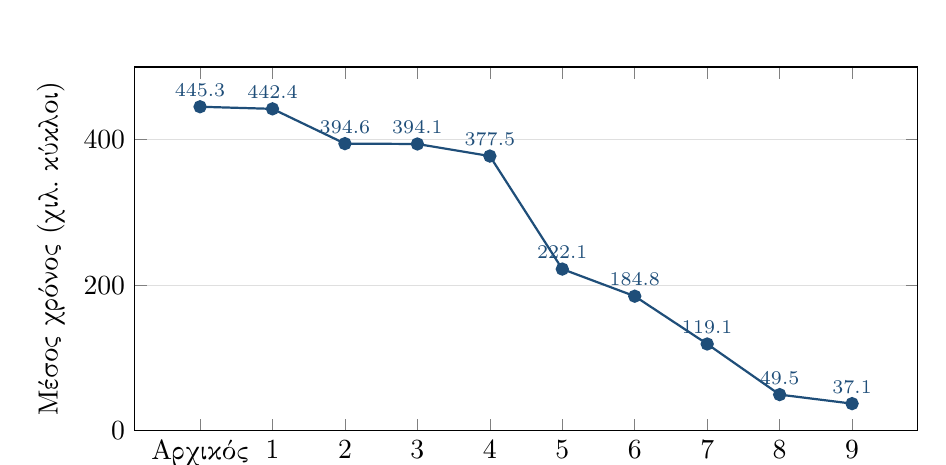
\begin{tikzpicture}
\begin{axis}[
  width=0.95\textwidth, height=6.2cm,
  symbolic x coords={v0,v1,v2,v3,v4,v5,v6,v7,v8,v9},
  xtick=data, xticklabels={Αρχικός,v1,v2,v3,v4,v5,v6,v7,v8,v9}, ymin=0, ymax=500,
  ylabel={Μέσος χρόνος (χιλ.\ κύκλοι)},
  ymajorgrids, grid style={gray!25},
  nodes near coords, every node near coord/.append style={font=\scriptsize, anchor=south},
  point meta=explicit symbolic]
\addplot[thick, color=accent, mark=*] coordinates {
  (v0,445.3)[445.3] (v1,442.4)[442.4] (v2,394.6)[394.6] (v3,394.1)[394.1] (v4,377.5)[377.5]
  (v5,222.1)[222.1] (v6,184.8)[184.8] (v7,119.1)[119.1] (v8,49.5)[49.5] (v9,37.1)[37.1]};
\end{axis}
\end{tikzpicture}
\caption{Εξέλιξη του μέσου χρόνου εκτέλεσης ανά έκδοση (Ερωτήματα 2--3).}
\label{fig:versions}
\end{figure}

\subsection{Συγκεντρωτικά Συμπεράσματα}
\begin{itemize}[leftmargin=*]
  \item \textbf{Οι βελτιώσεις που αφορούν τον εσωτερικό βρόχο οδηγεί σε σημαντικές βελτιώσεις.} Οι v1 και v3
  δίνουν μαζί $<1\%$. Οι v5, v7 και v8, που μειώνουν το κόστος \emph{ανά pixel}, δίνουν το $\sim$90\%
  του συνολικού κέρδους.
  \item \textbf{Ιεραρχία μνήμης:} η μετακίνηση των δεδομένων από flash σε SRAM (v7) είναι η μόνη
  βελτίωση που εκμεταλλεύεται άμεσα χαρακτηριστικό του \en{hardware}. Η v9 εκμεταλλεύεται
  αντίστοιχα το \en{ISA} (εντολές DSP).
  \item Συνολικά: \textbf{$12\times$ ταχύτερα} (v9) με πανομοιότυπα αποτελέσματα.
\end{itemize}

% ---------------------------------------------------------------------
\subsection{Ερώτημα 4}
% ---------------------------------------------------------------------

\subsubsection*{Πειραματική διαδικασία}
Ως βάση χρησιμοποιήθηκε η 8, η καλύτερη έκδοσή μας. Οι
κοινοί διαιρέτες των $N=M=10$ είναι $B\in\{1,2,5,10\}$. Για κάθε $B$ ο κώδικας έγινε compile με
διαφορετικό \code{\#define B} και εκτελέστηκε 10 φορές, διατηρώντας ως μετιρκή τον μέσο όρο.

\begin{table}[H]
\centering
\caption{DSE για τετραγωνικό μπλοκ. Η v8 είναι η βάση. Η v6 (δεδομένα στη flash) χρησιμοποιείται ως συμπληρωματικό πείραμα.}
\label{tab:dse_b}
\small
\begin{tabular}{@{}r rrrr c rr@{}}
\toprule
 & \multicolumn{4}{c}{\textbf{v8 (δεδομένα στη SRAM)}} & & \multicolumn{2}{c}{\textbf{v6 (δεδομένα στη flash)}} \\
\cmidrule(lr){2-5}\cmidrule(lr){7-8}
$B$ & \textbf{Μέσος} & \textbf{Min} & \textbf{Max} & \textbf{ms} & & \textbf{Μέσος} & \textbf{ms} \\
\midrule
1  & \num{125772.6} & \num{125772} & \num{125778} & \num{0.524053} & & \num{242610.2} & \num{1.010876} \\
2  & \num{71649.0}  & \num{71649}  & \num{71649}  & \num{0.298537} & & \num{199689.0} & \num{0.832038} \\
5  & \num{49504.0}  & \num{49504}  & \num{49504}  & \num{0.206267} & & \num{184796.5} & \num{0.769985} \\
10 & \textbf{\num{43655.0}} & \num{43655} & \num{43655} & \textbf{\num{0.181896}} & & \textbf{\num{181726.8}} & \textbf{\num{0.757195}} \\
\midrule
$T(1)/T(10)$ & \multicolumn{4}{c}{$2.88\times$} & & \multicolumn{2}{c}{$1.34\times$} \\
\bottomrule
\end{tabular}
\end{table}

\noindent\textbf{Βέλτιστο: $B=10$} και στις δύο εκδόσεις, δηλαδή το μεγαλύτερο δυνατό μπλοκ.

\begin{figure}[H]
\centering
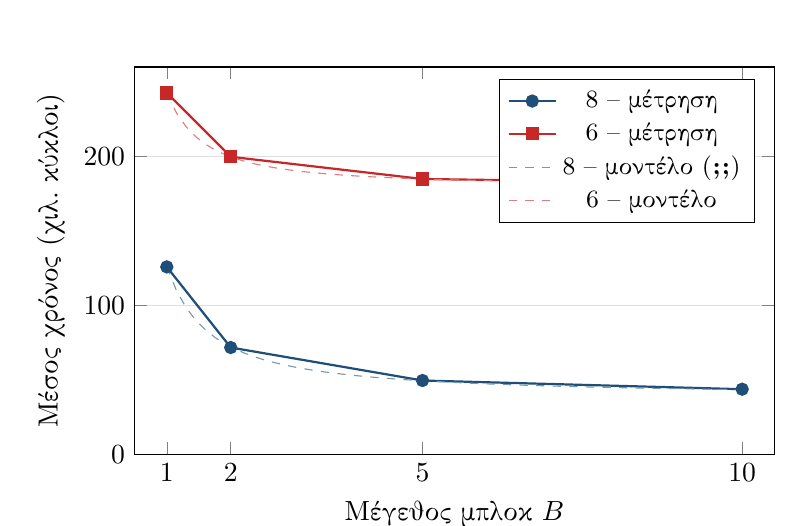
\begin{tikzpicture}
\begin{axis}[
  width=0.8\textwidth, height=6.5cm,
  xlabel={Μέγεθος μπλοκ $B$}, ylabel={Μέσος χρόνος (χιλ.\ κύκλοι)},
  xtick={1,2,5,10}, xmin=0.5, xmax=10.5, ymin=0, ymax=260,
  ymajorgrids, grid style={gray!25},
  legend pos=north east, legend style={font=\small}]
\addplot[thick, color=accent, mark=*] coordinates {(1,125.77) (2,71.65) (5,49.50) (10,43.66)};
\addlegendentry{v8 -- μέτρηση}
\addplot[thick, color=bad, mark=square*] coordinates {(1,242.61) (2,199.69) (5,184.80) (10,181.73)};
\addlegendentry{v6 -- μέτρηση}
\addplot[dashed, color=accent!60, domain=1:10, samples=60] {(38204 + 401.1*100/x^2 + 476.2*100/x)/1000};
\addlegendentry{v8 -- μοντέλο (\ref{eq:model})}
\addplot[dashed, color=bad!60, domain=1:10, samples=60] {(179484 + 454.9*100/x^2 + 176.3*100/x)/1000};
\addlegendentry{v6 -- μοντέλο}
\end{axis}
\end{tikzpicture}
\caption{Χρόνος εκτέλεσης συναρτήσει του $B$ (Ερώτημα 4). Οι διακεκομμένες είναι το αναλυτικό μοντέλο.}
\label{fig:dse_b}
\end{figure}

\subsubsection*{Block Size $B$ και Υπολογιστική Πολυπλοκότητα}

Υπολογίζουμε πόσες φορές εκτελείται κάθε επίπεδο
βρόχου της v8 (Πίνακας~\ref{tab:loop_levels}). Ο αριθμός blocks είναι $\frac{NM}{B_xB_y}$, και για
κάθε block εκτελούνται 3 βήματα ($S=4,2,1$) $\times$ 3 υποψήφιοι (\code{i\_loop(-S)},
\code{c\_loop}, \code{i\_loop(+S)}) $=9$ διπλοί βρόχοι $k,l$.

\begin{table}[H]
\centering
\caption{Συνολικές εκτελέσεις κάθε επιπέδου βρόχου της v8.}
\label{tab:loop_levels}
\small
\begin{tabularx}{\textwidth}{@{}l X c c c@{}}
\toprule
\textbf{Επίπεδο} & \textbf{Τι εκτελείται} & \textbf{Ανά μπλοκ} & \textbf{Σύνολο} & \textbf{Εξάρτηση} \\
\midrule
Σώμα του \code{l} &
  SAD: \code{d = cr[l]-pr[l]; dist += |d|} &
  $9B_xB_y$ & $9NM$ & σταθερό \\
Αντιγραφές &
  \code{prev\_pad[..] = previous[..]}, \code{cb[k][l] = current[..]} &
  -- & $2NM$ & σταθερό \\
\midrule
Σώμα του \code{k} &
  υπολογισμός \code{cr}, \code{pr}, \code{qr}, είσοδος/έξοδος του βρόχου \code{l} &
  $9B_x$ (+$B_x$ αντιγραφή) & $10\,\frac{NM}{B_y}$ & $\propto \frac{1}{B_y}$ \\
\midrule
Σώμα του \code{y} &
  \code{bx, by, vx, vy}, 9$\times$(\code{dist=0}, είσοδος στο \code{k}, συγκρίσεις min),
  3$\times$(\code{vx+=, vy+=}), αποθήκευση διανυσμάτων &
  1 & $\frac{NM}{B_xB_y}$ & $\propto \frac{1}{B_xB_y}$ \\
\bottomrule
\end{tabularx}
\end{table}

Όπως φαίνεται παραπάνω από το μπλοκ
εξαρτώνται μόνο τα \en{overheads}, δηλαδή πόσες φορές ξεκινά ο βρόχος \code{k} (μία ανά block) και
πόσες ο βρόχος \code{l} (μία ανά γραμμή block). Επομένως
\begin{equation}
T(B_x,B_y) \;=\; T_{\text{σταθ}} \;+\; O_{\text{μπλοκ}}\cdot\frac{NM}{B_xB_y} \;+\; O_{\text{γραμμής}}\cdot\frac{NM}{B_y},
\label{eq:model}
\end{equation}
όπου $O_{\text{μπλοκ}}$ και $O_{\text{γραμμής}}$ είναι το σταθερό κόστος σε κύκλους μιας εκτέλεσης του
σώματος του \code{y} και του \code{k} αντίστοιχα. Και οι δύο μεταβλητοί όροι \emph{φθίνουν} με τα
$B_x, B_y$, άρα ο χρόνος είναι μονότονα φθίνων και το βέλτιστο είναι πάντα το μεγαλύτερο επιτρεπτό
block. Επίσης, το $B_x$ απλοποιείται στον όρο γραμμής, γι' αυτό το $B_y$, δηλαδή το μήκος του εσωτερικού βρόχου, έχει
μεγαλύτερη επίδραση από το $B_x$.


\subsubsection*{Σύνδεση με χαρακτηριστικό του Hardaware}
Αρχικά, περιμέναμε το βέλτιστο $B$ να συνδέεται με την ιεραρχία
μνήμης. Για παράδειγμα, θα περιμέναμε ένα γόνατο στην καμπύλη χρόνου-block-size όταν το block παύει
να χωράει σε κάποια \en{cache}. Στη v8 όμως όλα τα δεδομένα της αναζήτησης ζουν στη SRAM, η οποία
δεν έχει \en{cache}. Η μόνη \en{cache} του S7G2 (FCACHE) αφορά τη flash, οπότε η v8 ουσιαστικά την
``παρακάμπτει''. Γι' αυτό επαναλάβαμε το ίδιο DSE στη \textbf{v6}, όπου οι εικόνες διαβάζονται
απευθείας από τη flash (μέσω FCACHE), με την ελπίδα να εμφανιστεί συμπεριφορά που να συνδέεται
πιο άμεσα με το \en{hardware}. Και εκεί όμως η καμπύλη είναι μονότονη.

Σε μια προσπάθεια να ερμηνεύσουμε αυτό το αποτέλεσμα καταλήξαμε στα παρακάτω:
\begin{enumerate}[leftmargin=*]
  \item \textbf{Το \en{working set} είναι μικροσκοπικό.} Με $N=M=10$ κάθε \en{frame} είναι
  $100\times\SI{4}{B}=\SI{400}{B}$. Μετά την πρώτη πρόσβαση όλα τα δεδομένα (και ο κώδικας του βρόχου)
  μένουν μόνιμα ``ζεστά'', ανεξάρτητα από το $B$. Δεν υπάρχουν \en{capacity/conflict misses} για να
  τα επηρεάσει το $B$. Αυτό επιβεβαιώνεται και από το ότι ούτε η πρώτη εκτέλεση είναι πιο αργή
  (min $\approx$ max).
  \item \textbf{Η πρόσβαση στη flash προσθέτει σταθερό κόστος ανά \en{pixel}.} Στη v6 ο όρος $c$ είναι
  $\approx 4.7\times$ μεγαλύτερος ($\approx\num{179500}$ έναντι \num{38200}), λόγω ελέγχων ορίων και
  αναγνώσεων από flash. Αυτός ο όρος \emph{δεν} εξαρτάται από το $B$ και απλώς ``αραιώνει'' την
  επίδραση των \en{overheads}: $T(1)/T(10)=1.34$ αντί για 2.88. Δεν δημιουργεί όμως ελάχιστο.
  \item \textbf{Το κυρίαρχο κόστος είναι λογισμικό.} Στο \code{-O0} κυριαρχούν οι \en{overheads}
  ελέγχου βρόχων. Η σύνδεση με το \en{hardware} περνάει μέσα από το \en{pipeline}: ο \en{Cortex-M4}
  έχει \en{pipeline} 3 σταδίων \emph{χωρίς} \en{branch predictor}, οπότε κάθε \en{taken branch}
  κοστίζει επιπλέον κύκλους για να ξαναγεμίσει το \en{pipeline}. Μεγαλύτερο $B$ σημαίνει λιγότερες
  είσοδοι/έξοδοι βρόχων και άρα λιγότερα \en{flushes}.
\end{enumerate}

\begin{insight}[Πώς θα μπορούσε να αναδειχθεί μια πραγματική σχέση με το \en{hardware}]
\begin{itemize}[leftmargin=*]
  \item \textbf{Μεγαλύτερο \en{frame}:} το \code{images.h} περιέχει \num{19200} τιμές ανά εικόνα
  ($\approx\SI{75}{KB}$), ενώ ο κώδικας χρησιμοποιεί μόνο τις πρώτες 100. Με π.χ.\ $N\times M=120\times160$
  (κοινοί διαιρέτες 1, 2, 4, 5, 8, 10, 20, 40), η v6 θα διάβαζε από τη flash δεδομένα πολύ μεγαλύτερα
  από τη FCACHE. Τότε το $B$ θα καθόριζε την επαναχρησιμοποίηση των γραμμών του παραθύρου
  $(B+2p)^2$ και θα μπορούσε να εμφανιστεί ``γόνατο''.
  \item \textbf{Απενεργοποίηση της FCACHE} (καταχωρητής \code{FCACHEE}) στη v6: η διαφορά on/off θα
  μετρούσε ευθέως τη συνεισφορά της.
  \item \textbf{Μεταγλώττιση με \code{-O2}:} οι όροι $a,b$ μικραίνουν δραστικά, οπότε τα φαινόμενα
  μνήμης γίνονται σχετικά πιο ορατά.
  \item \textbf{DSE πάνω στη v9:} εκεί αναμένεται εμφανής εξάρτηση από το \en{hardware}. Μπλοκ με $B_y$
  πολλαπλάσιο του 4 θα αξιοποιούσαν πλήρως το \code{USADA8} (4 \en{bytes} $=$ πλάτος καταχωρητή και
  \en{bus}). Με $N=M=10$ κανένας διαιρέτης δεν είναι πολλαπλάσιο του 4, γι' αυτό και δεν φαίνεται εδώ.
\end{itemize}
\end{insight}

\noindent Σημείωση: το $B=10$ σημαίνει ένα μόνο μπλοκ για όλο το \en{frame}, δηλαδή ένα διάνυσμα κίνησης.
Είναι το ταχύτερο, αλλά άχρηστο ως εκτίμηση κίνησης. Στην πράξη το $B$ επιλέγεται με κριτήριο
και την ποιότητα (π.χ.\ $8\times8$ ή $16\times16$ στα \en{codecs}), όχι μόνο την ταχύτητα.

% ---------------------------------------------------------------------
\subsection{Ερώτημα 5: \en{Design Space Exploration} για ορθογώνιο μπλοκ $B_x\times B_y$}
% ---------------------------------------------------------------------

\subsubsection*{Πειραματική διαδικασία}
Ίδια βάση (v8), όπου πλέον \code{Bx} (γραμμές, διαιρέτης του $N$) και \code{By} (στήλες, διαιρέτης
του $M$) είναι ανεξάρτητα \code{\#define}. Εξετάστηκαν εξαντλητικά και τα $4\times4=16$ ζεύγη
$B_x,B_y\in\{1,2,5,10\}$, με 10 εκτελέσεις το καθένα. Οι 4 διαγώνιες τιμές συμπίπτουν με το Ερώτημα~4.

\begin{table}[H]
\centering
\caption{Μέσος χρόνος (κύκλοι) για κάθε ζεύγος $(B_x,B_y)$, v8. Πιο σκούρο χρώμα σημαίνει ταχύτερη εκτέλεση.}
\label{tab:dse_bxby}
\begin{tabular}{@{}c|rrrr@{}}
\toprule
$B_x \backslash B_y$ & \textbf{1} & \textbf{2} & \textbf{5} & \textbf{10} \\
\midrule
\textbf{1}  & \num{125772.6} & \cellcolor{accent!5}\num{82182.2}  & \cellcolor{accent!25}\num{55917.2} & \cellcolor{accent!40}\num{46805.4} \\
\textbf{2}  & \num{106274.2} & \cellcolor{accent!10}\num{71649.0} & \cellcolor{accent!30}\num{51912.2} & \cellcolor{accent!45}\num{44822.8} \\
\textbf{5}  & \cellcolor{accent!2}\num{93971.0}  & \cellcolor{accent!15}\num{65687.4} & \cellcolor{accent!35}\num{49504.0} & \cellcolor{accent!50}\num{43692.1} \\
\textbf{10} & \cellcolor{accent!3}\num{89846.4}  & \cellcolor{accent!18}\num{63663.0} & \cellcolor{accent!38}\num{48761.1} & \cellcolor{accent!60}\textbf{\num{43655.0}} \\
\bottomrule
\end{tabular}
\end{table}

\begin{figure}[H]
\centering
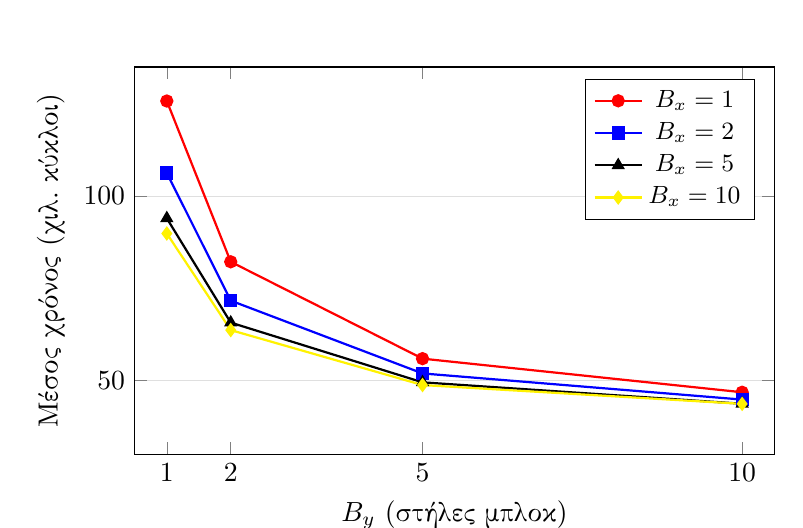
\begin{tikzpicture}
\begin{axis}[
  width=0.8\textwidth, height=6.5cm,
  xlabel={$B_y$ (στήλες μπλοκ)}, ylabel={Μέσος χρόνος (χιλ.\ κύκλοι)},
  xtick={1,2,5,10}, xmin=0.5, xmax=10.5, ymin=30, ymax=135,
  ymajorgrids, grid style={gray!25},
  legend pos=north east, legend style={font=\small}, cycle list name=color list]
\addplot+[thick, mark=*] coordinates {(1,125.77) (2,82.18) (5,55.92) (10,46.81)};
\addlegendentry{$B_x=1$}
\addplot+[thick, mark=square*] coordinates {(1,106.27) (2,71.65) (5,51.91) (10,44.82)};
\addlegendentry{$B_x=2$}
\addplot+[thick, mark=triangle*] coordinates {(1,93.97) (2,65.69) (5,49.50) (10,43.69)};
\addlegendentry{$B_x=5$}
\addplot+[thick, mark=diamond*] coordinates {(1,89.85) (2,63.66) (5,48.76) (10,43.66)};
\addlegendentry{$B_x=10$}
\end{axis}
\end{tikzpicture}
\caption{Χρόνος εκτέλεσης συναρτήσει του $B_y$, για κάθε $B_x$ (Ερώτημα 5).}
\label{fig:dse_bxby}
\end{figure}

\noindent\textbf{Βέλτιστο ζεύγος: $(B_x,B_y)=(10,10)$} με \num{43655} κύκλους (\SI{0.1819}{ms}). Πολύ
κοντά ακολουθεί το $(5,10)$ με \num{43692} κύκλους (διαφορά 0.08\%).

\subsubsection*{Σχολιασμός}
Το $B_y$ επηρεάζει τον χρόνο πολύ περισσότερο από το $B_x$. Για ίδιο εμβαδόν μπλοκ,
το $(1,2)$ χρειάζεται \num{82182} κύκλους και το $(2,1)$ \num{106274}, δηλαδή 29\% περισσότερους.
Αυτό εξηγείται άμεσα από την ανάλυση που κάναμε στο προηγούμενο ερώτημα. Εκεί αποδείχθηκε ότι ο όρος $b\,NM/B_y$ εξαρτάται μόνο από το $B_y$. Κάθε γραμμή block πληρώνει μία φορά τον
υπολογισμό δεικτών και το \en{overhead} του βρόχου $l$. Επιπλέον, το $B_y$ αντιστοιχεί στη διάσταση
που είναι συνεχόμενη στη μνήμη.

Το $B_x$, από την άλλη, επηρεάζει μόνο τον όρο ($a\,NM/(B_xB_y)$), ο οποίος γίνεται αμελητέος όταν το
$B_y$ είναι μεγάλο. Γι' αυτό οι καμπύλες συγκλίνουν στο $B_y=10$ (\num{46805}$\to$\num{43655}).

Συνολικά με βάση και την ανάλυση στο ερώτημα 4, παρατηρείται βέλτιστη απόδοση στις μεγαλύτερες τιμές των $Bx$ και $By$, με την ιεραρχία της μνήμης να μην διαδραμτίζει καθοριστικό ρόλο.

\begin{insight}[Ευριστικός περιορισμός της αναζήτησης]
Αφού το $T$ είναι \textbf{μονότονα φθίνον και ως προς τα δύο ορίσματα και (σχεδόν) διαχωρίσιμο}, δεν
χρειάζεται εξαντλητική αναζήτηση $|D(N)|\cdot|D(M)|$:
\begin{enumerate}[leftmargin=*]
  \item \textbf{Πρώτα ο κυρίαρχος άξονας:} σταθεροποιούμε το $B_x$ και σαρώνουμε το $B_y$ (που έχει το
  μεγαλύτερο βάρος). Μετά σαρώνουμε το $B_x$ με το καλύτερο $B_y$ (\en{coordinate descent}). Χρειάζονται
  $|D(N)|+|D(M)|-1=7$ αξιολογήσεις αντί για 16. Για μεγάλα \en{frames} το κέρδος γίνεται πολύ μεγαλύτερο: για $144\times176$ (QCIF, 15 και 10 διαιρέτες)
  χρειάζονται 24 αξιολογήσεις αντί για 150.
  \item \textbf{Αναζήτηση με μοντέλο:} με 3 μόνο μετρήσεις εκτιμώνται τα $a,b,c$ της~(\ref{eq:model}) και
  προβλέπεται όλος ο χώρος. Εδώ το σφάλμα πρόβλεψης ήταν $<0.7\%$.
  \item \textbf{Περιορισμοί από το \en{hardware} και την ποιότητα:} προτιμούμε $B_y$ πολλαπλάσιο του 4 (για
  SIMD) και απορρίπτουμε εκ των προτέρων μπλοκ τόσο μεγάλα που να μη δίνουν χρήσιμα διανύσματα κίνησης.
\end{enumerate}
\end{insight}

\newpage
% =====================================================================
\section{Ζητούμενο 2ο}
% =====================================================================

% ---------------------------------------------------------------------
\subsection{Ερώτημα 1}
% ---------------------------------------------------------------------
Έγινε η παρακάτω τροποποίηση στο αρχείο \code{simple.py} προκειμένου να διαβάζει το εκτελέσιμο από
την γραμμή εντολών.

\begin{figure}[H]
\centering
\begin{subfigure}[b]{0.42\textwidth}
  \centering
  \includegraphics[width=\textwidth]{figures/z2/simple_before.png}
  \caption{Από}
\end{subfigure}\hfill
\begin{subfigure}[b]{0.52\textwidth}
  \centering
  \includegraphics[width=\textwidth]{figures/z2/simple_after.png}
  \caption{Σε}
\end{subfigure}
\caption{Τροποποίηση του \code{simple.py}.}
\end{figure}

Μετά την εκτέλεση της προσομοίωσης οι συνολικοί κύκλοι που υπολογίστηκαν είναι \textbf{\num{857689669}}:

\begin{figure}[H]
\centering
\includegraphics[width=\textwidth]{figures/z2/cycles_simple.png}
\caption{\code{system.cpu.numCycles} για την πρώτη αρχιτεκτονική.}
\end{figure}

% ---------------------------------------------------------------------
\subsection{Ερώτημα 2}
% ---------------------------------------------------------------------
Μετά την εκτέλεση της προσομοίωσης της δεύτερης αρχιτεκτονικής οι συνολικοί κύκλοι που υπολογίστηκαν
είναι \textbf{\num{59787087}}:

\begin{figure}[H]
\centering
\includegraphics[width=\textwidth]{figures/z2/cycles_twolevel.png}
\caption{\code{system.cpu.numCycles} για τη δεύτερη αρχιτεκτονική (L1I = L1D = \SI{8}{kB}, L2 = \SI{128}{kB}).}
\end{figure}

\subsubsection*{Σύγκριση -- Εξήγηση}
Παρατηρούμε ότι οι συνολικοί κύκλοι που απαιτούνται για την εκτέλεση του ίδιου εκτελέσιμου είναι μια
τάξη μεγέθους μικρότεροι στην δεύτερη αρχιτεκτονική, οδηγώντας σε συνολικό speed-up $\num{857689669}/\num{59787087}\approx\mathbf{14.3\times}$. Αυτή η δραματική μείωση οφείλεται στην σύνθετη
ιεραρχία μνήμης της δεύτερης αρχιτεκτονικής. Σε αυτήν, υπάρχουν μικρά \en{modules} μνήμης \en{on chip}
(\en{cache memories}) οι οποίες εξαλείφουν σημαντικά το \en{latency} μεταφοράς δεδομένων που εισάγει η
κύρια μνήμη. Επομένως η πρώτη αρχιτεκτονική αλληλεπιδρά αποκλειστικά με την μνήμη RAM, ενώ η δεύτερη
-- παρά τις αναπόφευκτες προσβάσεις στην μνήμη RAM -- επωφελείται από τον σημαντικό αριθμό
\en{cache hits} μειώνοντας δραστικά το χρονικό κόστος αναμονής δεδομένων από την μνήμη. Α


% ---------------------------------------------------------------------
\subsection{Ερώτημα 3}
% ---------------------------------------------------------------------

\subsubsection*{Επιρροή \en{unrolling factor}}

\begin{figure}[H]
\centering
\includegraphics[width=0.75\textwidth]{figures/z2/plot_uf.png}
\caption{Κύκλοι συναρτήσει του \en{unrolling factor} (L1I = L1D = \SI{8}{kB}, L2 = \SI{128}{kB}).}
\label{fig:uf}
\end{figure}

% TODO: (προαιρετικά) πίνακας με τις ακριβείς τιμές του γραφήματος, π.χ.:
% \begin{table}[H]\centering
% \begin{tabular}{@{}rr@{}}\toprule UF & Κύκλοι \\ \midrule
% 2 & ... \\ 4 & ... \\ 8 & ... \\ 16 & ... \\ 32 & ... \\ \bottomrule\end{tabular}
% \end{table}

\subsection*{Παρουσίαση -- Εξήγηση.}
Στο παραπάνω γράφημα παρατηρούμε ότι η αύξηση του \en{unrolling factor} οδηγεί σε βελτίωση της χρονικής
επίδοσης του κώδικα μέχρι και το \en{unrolling\_factor} = 16, όπου έχουμε και την καλύτερη επίδοση
συνολικά. Ωστόσο περαιτέρω αύξηση του \en{unrolling factor} φαίνεται πως οδηγεί σε αύξηση των συνολικών
κύκλων.

Η αρχική μείωση των συνολικών κύκλων με την αύξηση του \en{unrolling factor} είναι αναμενόμενη καθώς με
αυτόν τον τρόπο ελαχιστοποιείται το \en{branch penalty} (το σώμα του \en{loop} εκτελείται λιγότερες φορές,
συνεπώς μειώνονται οι έλεγχοι για \en{jumps}, έχουμε λιγότερη χρήση του \en{branch predictor} και
αποφυγή των \en{mispredictions}). Επιπλέον μέσα στο σώμα του \en{loop} προκύπτουν περισσότερες ανεξάρτητες
εντολές οι οποίες δύναται να εκτελεστούν παράλληλα μέσω τεχνικών παραλληλισμού (SIMD), όπως το
\en{vectorization}. Η συγκεκριμένη μορφή κώδικα στο αρχείο \code{tables.exe} επιτρέπει μαζικό
παραλληλισμό λόγω της απουσίας εξαρτήσεων μεταξύ των εντολών μέσα στο βρόχο.

Ωστόσο η συνεχής αύξηση του \en{unrolling factor} δεν είναι πανάκεια, όπως φαίνεται για UF=32 όπου έχουμε
και αύξηση των κύκλων. Αυτό διότι με την αύξηση των εντολών που εκτελούνται σε ένα \en{iteration}
αυξάνεται ταυτόχρονα και η ανάγκη για \en{registers} που αποθηκεύουν \en{temporary variables}. Λόγω του
περιορισμένου αριθμού από \en{registers} ορισμένες από αυτές τις προσωρινές μεταβλητές πρέπει να
αποθηκευτούν στην \en{stack} εισάγοντας έτσι καθυστερήσεις.

\begin{insight}
Το εύρος της μεταβολής είναι μικρό: από UF=2 σε UF=16 οι κύκλοι μειώνονται κατά $\sim$0.7\%. Ο βρόχος
είναι \en{memory-bound}, άρα ο \en{overhead} ελέγχου που αφαιρεί το \en{unrolling} είναι μικρό
κλάσμα του συνολικού χρόνου. Επιπλέον, για UF=32 το σώμα του βρόχου μεγαλώνει πολύ και ασκεί
πίεση στην L1I των \SI{8}{kB}. Ενδεικτικό είναι ότι στο Pareto μέτωπο του Ερωτήματος~4 (Πίνακας~\ref{tab:pareto_ex}), όταν η L1I
είναι μόλις \SI{2}{kB} επιλέγεται πάντα UF=8 αντί για UF=16. Με πολύ μικρή \en{instruction cache} το
μεγαλύτερο ξεδιπλωμένο σώμα παύει να χωράει.
\end{insight}

\subsubsection*{Επιρροή L1 \en{data cache size}}

\begin{figure}[H]
\centering
\includegraphics[width=0.75\textwidth]{figures/z2/plot_l1d.png}
\caption{Κύκλοι συναρτήσει του μεγέθους της L1D (L1I = \SI{8}{kB}, L2 = \SI{128}{kB}).}
\label{fig:l1d}
\end{figure}

\paragraph{Παρουσίαση -- Εξήγηση.}
Από το γράφημα γίνεται αντιληπτό ότι η αύξηση του μεγέθους της L1 \en{data cache} κάτω από ένα κρίσιμο
συνολικό μέγεθος δεν προσφέρει τίποτα παρά μια ελάχιστη βελτίωση στον χρόνο εκτέλεσης του κώδικα.
Ωστόσο η μετάβαση από τα \SI{8}{kB} στα \SI{16}{kB} βελτιώνει την επίδοση δραματικά. Η περαιτέρω αύξηση
στα \SI{32}{kB} προσφέρει μείωση των συνολικών κύκλων, αλλά όχι της ίδιας δυναμικής της προηγούμενης
μετάβασης, ενώ η αύξηση στα \SI{64}{kB} λειτουργεί αντίστροφα στην επίδοση, αυξάνοντας τους συνολικούς
κύκλους.

Σε μια πρώτη προσπάθεια ερμηνείας του διαγράμματος θεωρήσαμε ότι στις μνήμες μέχρι \SI{8}{kB} υπάρχει
άμεσο \en{aliasing}, δηλαδή ότι οι διευθύνσεις των στοιχείων κάθε πίνακα σε ένα \en{iteration}
(\code{x1[i], x2[i], x3[i], y[i]}) προβάλλονται στα ίδια \en{sets} οδηγώντας σε πολλά \en{conflicts} και μη
αξιοποίηση της χωρικής τοπικότητας. Ωστόσο μετά από μελέτη των αντίστοιχων αρχείων
(\code{two\_level.py}, \code{caches.py}, \code{tables.c}) καταλάβαμε ότι αυτό το \en{aliasing} βάσει του
πλήθους των στοιχείων κάθε πίνακα δεν υφίσταται ούτε σε αυτές τις μνήμες. Επομένως προχωρήσαμε σε μια
εναλλακτική πιθανή αιτιολόγηση για το άλμα στην μετάβαση από \SI{8}{kB} σε \SI{16}{kB}.

Με βάση τα αρχεία διαμόρφωσης του προσομοιωτή, η L1 \en{Data Cache} έχει \en{2-way associativity},
μέγεθος \en{block} 64 \en{bytes} (ικανό να φιλοξενήσει 8 μεταβλητές \code{double}) και διαθέτει 4
MSHRs. Ο συνδυασμός αυτών των παραμέτρων με τους τέσσερις πίνακες των \num{800000} \en{bytes} καθορίζει
επακριβώς τη συμπεριφορά της μνήμης σε κάθε φάση του διαγράμματος.

Στη ζώνη των \SI{2}{kB} έως \SI{8}{kB}, η απόδοση πέφτει λόγω του έντονου \en{cache thrashing}, το
οποίο προκαλείται από την μικρή απόσταση των δεδομένων στην \en{cache}. Ειδικά στα \SI{8}{kB}, η
\en{cache} διαθέτει μόλις 64 \en{sets}. Με βάση τα \en{offsets} των πινάκων, οι αρχικές τους διευθύνσεις
κατανέμονται ως εξής: ο \code{x1} στο \en{set} 0, ο \code{x2} στο \en{set} 20, ο \code{x3} στο
\en{set} 40 και ο \code{y} στο \en{set} 60. Παρόλο που οι πίνακες δεν αντιστοιχίζονται στο ίδιο ακριβώς
\en{set} για να προκαλέσουν άμεσο \en{aliasing}, η απόσταση μεταξύ τους είναι εξαιρετικά μικρή (ο
πίνακας \code{y} απέχει κυκλικά μόλις 4 \en{sets} από τον \code{x1}). Καθώς ο βρόχος εκτελείται, ο
\en{prefetcher} του επεξεργαστή σπεύδει να φέρει προκαταβολικά στην \en{cache} πολλαπλά επόμενα
\en{blocks} για κάθε πίνακα. Αυτή η διαδικασία οδηγεί τα \en{prefetched blocks} του \code{y} να
συγκρούονται με τα \en{blocks} του \code{x1}, αντικαθιστώντας τα ενεργά του δεδομένα, ενώ ταυτόχρονα τα
\en{prefetched blocks} των \code{x1} και \code{x2} συγκρούονται στην πορεία.

Το μεγάλο άλμα απόδοσης στα \SI{16}{kB} οφείλεται στην επίλυση αυτών των συγκρούσεων μέσω της
διεύρυνσης του διαθέσιμου χώρου. Με 128 διαθέσιμα \en{sets}, ο \code{x1} παραμένει στο \en{set} 0, ο
\code{x3} τοποθετείται στο 40, ο \code{x2} στο 84 και ο \code{y} στο 124. Αν και ο \code{y} εξακολουθεί
να βρίσκεται κοντά στον \code{x1}, ο διπλασιασμός των συνολικών \en{sets} αραιώνει τις αποστάσεις των
απεικονίσεων για τους υπόλοιπους πίνακες. Ο \en{prefetcher} μπορεί πλέον να φέρνει και να διατηρεί
ταυτόχρονα τις ενεργές γραμμές μνήμης και για τους τέσσερις πίνακες, χωρίς μαζικά \en{conflicts}. Το
\en{spatial locality} αξιοποιείται πλήρως, καθώς ένα \en{block} 64 \en{bytes} προσφέρει 7 συνεχόμενα
\en{cache hits} χωρίς να διαγράφεται πρόωρα.

Φτάνοντας στα \SI{32}{kB}, το σύστημα συναντά το ιδανικό σημείο ισορροπίας. Τα 256 \en{sets}
διασκορπίζουν τις απεικονίσεις των δεδομένων τόσο μακριά την μία από την άλλη, που εγγυώνται την
απόλυτη απουσία \en{conflict misses} κατά τη διάρκεια του βρόχου.

Η περαιτέρω αύξηση του μεγέθους στα \SI{64}{kB} οδηγεί σε μείωση της απόδοσης. Τα \en{conflict misses}
(που αποτελούν το μεγαλύτερο ποσοστό των συνολικών \en{misses}) έχουν ήδη εξαλειφθεί στα \SI{32}{kB}. Η
επιπλέον χωρητικότητα, ναι μεν μειώνει περαιτέρω τα \en{capacity misses}, αυξάνει δε το \en{overhead}
της \en{cache}, δηλαδή τον χρόνο αποκωδικοποίησης των διευθύνσεων λόγω των μεγαλύτερων
\en{critical paths}.

% ---------------------------------------------------------------------
\subsection{Ερώτημα 4: Εξαντλητική αναζήτηση και Pareto μέτωπο}
% ---------------------------------------------------------------------

\begin{figure}[H]
\centering
\includegraphics[width=\textwidth]{figures/z2/pareto_exhaustive.png}
\caption{Όλα τα 720 σημεία του χώρου σχεδίασης και το Pareto μέτωπο της εξαντλητικής αναζήτησης.}
\label{fig:pareto_ex}
\end{figure}

Δημιουργήθηκε κατάλληλο \en{python script} για την αυτόματη εκτέλεση της προσομοίωσης για όλες τις
δυνατές παραμετροποιήσεις του \en{search space} (L1D, L1I, L2, UF). Στο αρχείο
\code{all\_simulation\_results.csv} καταγράφεται το πλήθος των κύκλων για την εκτέλεση της εφαρμογής με
κάθε μια από τις δυνατές παραμετροποιήσεις. Ο κώδικας \en{python} υπολόγισε τον συνολικό χρόνο που
απαιτήθηκε για την εξαντλητική αναζήτηση των 720 εκδοχών στα 105 λεπτά όπως φαίνεται και παρακάτω:

\begin{figure}[H]
\centering
\includegraphics[width=0.85\textwidth]{figures/z2/exhaustive_time_crop.png}
\caption{Συνολικός χρόνος εξαντλητικής αναζήτησης (\SI{6306.95}{s} $\approx$ 105 λεπτά).}
\end{figure}

Επιπλέον ο κώδικας μέσω της βιβλιοθήκης \code{paretoset} υπολόγισε το \en{pareto frontier}, τα σημεία
του οποίου παρουσιάζονται στον Πίνακα~\ref{tab:pareto_ex} και καταγράφονται στο αρχείο
\code{pareto\_frontier\_results.csv}.

\begin{table}[H]
\centering
\caption{Pareto-βέλτιστα σημεία της εξαντλητικής αναζήτησης (20 σημεία).}
\label{tab:pareto_ex}
\small
\begin{tabular}{@{}rrrrrr@{}}
\toprule
\textbf{L1D (kB)} & \textbf{L1I (kB)} & \textbf{L2 (kB)} & \textbf{UF} & \textbf{totalMemoryKB} & \textbf{latencyCC} \\
\midrule
2  & 2  & 128 & 8  & 132 & \num{59581198} \\
4  & 2  & 128 & 8  & 134 & \num{59433698} \\
4  & 4  & 128 & 16 & 136 & \num{59343511} \\
8  & 4  & 128 & 16 & 140 & \num{59306017} \\
8  & 8  & 128 & 16 & 144 & \num{59296471} \\
\rowcolor{accent!8}
16 & 2  & 128 & 8  & 146 & \num{42416612} \\
16 & 4  & 128 & 16 & 148 & \num{42409832} \\
16 & 8  & 128 & 16 & 152 & \num{42403308} \\
16 & 16 & 128 & 16 & 160 & \num{42387518} \\
32 & 2  & 128 & 8  & 162 & \num{42078234} \\
32 & 4  & 128 & 16 & 164 & \num{41969420} \\
32 & 8  & 128 & 16 & 168 & \num{41969226} \\
32 & 16 & 128 & 16 & 176 & \num{41945801} \\
32 & 32 & 128 & 16 & 192 & \num{41936488} \\
32 & 16 & 256 & 16 & 304 & \num{41933039} \\
32 & 64 & 256 & 16 & 352 & \num{41928359} \\
64 & 64 & 256 & 16 & 384 & \num{41925024} \\
32 & 16 & 512 & 16 & 560 & \num{41923846} \\
32 & 32 & 512 & 16 & 576 & \num{41923699} \\
64 & 16 & 512 & 16 & 592 & \num{41922998} \\
\bottomrule
\end{tabular}
\end{table}

\begin{insight}
\begin{itemize}[leftmargin=*]
  \item Το μέτωπο έχει ένα σαφές ``γόνατο'' (χρωματισμένη γραμμή). Προσθέτοντας μόλις \SI{2}{kB}
  συνολικής μνήμης (144$\to$\SI{146}{kB}, με L1D $8\to16$\,kB) οι κύκλοι πέφτουν κατά \textbf{28\%}. Είναι
  η ίδια μετάβαση με το Σχήμα~\ref{fig:l1d}. Από τα \SI{176}{kB} έως τα \SI{592}{kB}, δηλαδή με
  $3.4\times$ περισσότερη μνήμη, το συνολικό κέρδος είναι μόλις 0.05\%. Τα σημεία αυτά είναι
  τυπικά Pareto-βέλτιστα, αλλά πρακτικά δεν έχουν αξία.
  \item Ο Πίνακας ταξινομήθηκε κατά αύξουσα μνήμη. Σε ένα Pareto μέτωπο δύο στόχων, η αύξηση της μνήμης
  συνοδεύεται πάντα από μείωση των κύκλων.
\end{itemize}
\end{insight}

% ---------------------------------------------------------------------
\subsection{Ερώτημα 5: Αναζήτηση με γενετικό αλγόριθμο (NSGA-II)}
% ---------------------------------------------------------------------
Ο δοσμένος κώδικας \code{genOptimizer.py} τροποποιήθηκε κατάλληλα για να καταγράφει τον συνολικό
αριθμό \en{evaluations} και τον συνολικό χρόνο της αναζήτησης, όπως φαίνεται παρακάτω:

\begin{figure}[H]
\centering
\includegraphics[width=0.9\textwidth]{figures/z2/genopt_code.png}
\caption{Τροποποίηση του \code{genOptimizer.py} για τη μέτρηση χρόνου και \en{evaluations}.}
\end{figure}

Μετά την εκτέλεση του παραπάνω \en{script} προέκυψαν τα σημεία του \en{pareto frontier} που φαίνονται
στον παρακάτω πίνακα και καταγράφονται στο αρχείο \code{genOptimizer\_PO.csv}. Επίσης υπολογίζονται τα
συνολικά \en{evaluations} και ο συνολικός χρόνος αναζήτησης στις τιμές \textbf{30} και
\textbf{\SI{254.53}{sec}} αντίστοιχα, όπως φαίνεται και παρακάτω:

\begin{figure}[H]
\centering
\includegraphics[width=\textwidth]{figures/z2/genopt_output.png}
\caption{Έξοδος του \code{genOptimizer.py}.}
\end{figure}

\begin{table}[H]
\centering
\caption{Pareto-βέλτιστα σημεία του γενετικού αλγορίθμου (ταξινομημένα κατά μνήμη).}
\label{tab:pareto_ga}
\small
\begin{tabular}{@{}rrrrrr c@{}}
\toprule
\textbf{L1I} & \textbf{L1D} & \textbf{L2} & \textbf{UF} & \textbf{exec\_time\_cc} & \textbf{total\_mem\_kB} & \textbf{Στο πραγματικό μέτωπο;} \\
\midrule
2kB  & 2kB  & 128kB & 8  & \num{59581198} & 132 & \textcolor{good}{\checkmark} \\
4kB  & 4kB  & 128kB & 16 & \num{59343511} & 136 & \textcolor{good}{\checkmark} \\
8kB  & 8kB  & 128kB & 16 & \num{59296471} & 144 & \textcolor{good}{\checkmark} \\
8kB  & 32kB & 128kB & 16 & \num{41969226} & 168 & \textcolor{good}{\checkmark} \\
\rowcolor{bad!8}
32kB & 64kB & 256kB & 16 & \num{41929862} & 352 & \textcolor{bad}{$\times$} \\
64kB & 64kB & 256kB & 16 & \num{41925024} & 384 & \textcolor{good}{\checkmark} \\
\bottomrule
\end{tabular}
\end{table}

Παράγουμε επίσης το \en{plot} με το σύνολο των σημείων του χώρου αναζήτησης και σχεδιασμένο το
\en{pareto frontier} όπως αυτό προκύπτει από τα σημεία που επιστρέφει ο \en{heuristic algorithm}.

\begin{figure}[H]
\centering
\includegraphics[width=\textwidth]{figures/z2/pareto_ga.png}
\caption{Pareto μέτωπο του NSGA-II πάνω στο σύνολο του χώρου σχεδίασης.}
\end{figure}

\subsubsection*{Σχολιασμός}
Ο \en{heuristic} αλγόριθμος εξετάζει ένα σημαντικά μικρότερο υποσύνολο των πιθανών διατάξεων (30 vs 720)
οδηγώντας όπως είναι αναμενόμενο σε δραματικά λιγότερο χρόνο (\SI{254}{sec} vs 105 \en{min}, δηλαδή
$\sim$25$\times$ ταχύτερη αναζήτηση). Αυτή η μείωση των απαιτήσεων σε χρόνο προκύπτει ως απόρροια των
παραμέτρων του αλγορίθμου (\code{n\_max\_gen=5} και \code{n\_offspring=5}). Βάσει αυτών ο αλγόριθμος θα
εκτελέσει το πολύ 35 αξιολογήσεις (10 για τον αρχικό πληθυσμό και 25 για τις 5 επόμενες γενιές), τη
στιγμή που η εξαντλητική αναζήτηση απαιτεί 720.

Για να επιτευχθεί αυτός ο μικρότερος χρόνος θυσιάζεται αντίστοιχα η ακρίβεια στην εύρεση των σημείων
του \en{pareto frontier}. Για την σύγκριση των \en{pareto frontier points} του \en{heuristic algorithm} με
τα \en{ground truth} σημεία από το \en{exhaustive search}, αναπτύχθηκε κώδικας \en{python} που υπολογίζει
διάφορες ποιοτικές μετρικές όπως φαίνεται στην παρακάτω εικόνα:

\begin{figure}[H]
\centering
\includegraphics[width=0.65\textwidth]{figures/z2/pareto_metrics.png}
\caption{Μετρικές ποιότητας του μετώπου του NSGA-II σε σχέση με το πραγματικό μέτωπο.}
\end{figure}

Παρατηρούμε ότι ο \en{heuristic algorithm} κατάφερε να αναγνωρίσει μόνο 5 από τα πραγματικά
\en{pareto frontier points}, παρέλειψε τα υπόλοιπα 15, ενώ ανέδειξε ένα ψευδές σημείο ως
\en{pareto frontier point}.

Γνωρίζουμε ότι ο αλγόριθμος NSGA-II δεν εγγυάται πως θα βρει το αληθινό μέτωπο, καθώς παραμένει μια
στοχαστική μέθοδος. Ωστόσο, προσφέρει μια αρκετά αποτελεσματική μέθοδο για τον ποιοτικό και όσο το
δυνατόν ακριβέστερο προσδιορισμό του μετώπου. Χάρη στον μηχανισμό \en{elitism}, οι λύσεις δεν
υποβαθμίζονται ποτέ, και χάρη στο \en{crowding distance}, καλύπτουν όλο το εύρος των \en{trade-offs}
μεταξύ χρόνου και μνήμης.

\begin{insight}
\begin{itemize}[leftmargin=*]
  \item \textbf{Το ψευδές σημείο} είναι το (L1I=32, L1D=64, L2=256, UF=16) με \SI{352}{kB}/\num{41929862}
  κύκλους. Κυριαρχείται από το (L1I=64, L1D=32, L2=256, UF=16) του πραγματικού μετώπου, που έχει
  \emph{ίδια} μνήμη (\SI{352}{kB}) και \num{1503} λιγότερους κύκλους. Απλώς ο GA δεν αξιολόγησε ποτέ τη
  διάταξη αυτή, άρα ``ψευδές'' σημαίνει ``βέλτιστο μεταξύ όσων είδε''.
  \item \textbf{Υψηλή \en{precision} (83\%), χαμηλό \en{recall} (25\%):} με 30 αξιολογήσεις ο GA
  βρίσκει σωστά τα ``ακραία'' και πιο ενδιαφέροντα σημεία, όπως το γόνατο στα \SI{168}{kB}, αλλά δεν
  έχει τον προϋπολογισμό να γεμίσει τις ενδιάμεσες, σχεδόν ισοδύναμες λύσεις.
  \item Η πρακτική απώλεια είναι μικρή. Το καλύτερο σημείο του GA είναι μόλις 0.005\% πιο αργό από το
  πραγματικό βέλτιστο (\num{41925024} έναντι \num{41922998} κύκλων), με $\sim$4\% του κόστους αναζήτησης.
\end{itemize}
\end{insight}

% =====================================================================
\appendix
\section{Παράρτημα: \en{Screenshots} μετρήσεων (Ζητούμενο 1)}
\label{app:z1}
% =====================================================================

Όλες οι τιμές διαβάστηκαν από το \en{Expressions view} του \en{e2studio} μετά το τέλος των 10 εκτελέσεων.

\newcommand{\shot}[2]{%
  \begin{subfigure}[t]{0.32\textwidth}\centering
  \includegraphics[width=\textwidth]{#1}\caption{#2}\end{subfigure}}

\begin{figure}[H]
\centering
\shot{figures/z1/q2_base.png}{Αρχικός κώδικας}
\caption{Ερώτημα 2: μέτρηση του αρχικού κώδικα.}
\label{fig:app_q2}
\end{figure}

\begin{figure}[H]
\centering
\shot{figures/z1/q3_v1.png}{v1}\hfill
\shot{figures/z1/q3_v2.png}{v2}\hfill
\shot{figures/z1/q3_v3.png}{v3}\\[4pt]
\shot{figures/z1/q3_v4.png}{v4}\hfill
\shot{figures/z1/q3_v5.png}{v5}\hfill
\shot{figures/z1/q3_v6.png}{v6}\\[4pt]
\shot{figures/z1/q3_v7.png}{v7}\hfill
\shot{figures/z1/q3_v8.png}{v8}\hfill
\shot{figures/z1/q3_v9.png}{v9}
\caption{Ερώτημα 3: μετρήσεις των εκδόσεων v1--v9 ($B=5$).}
\end{figure}

\begin{figure}[H]
\centering
\shot{figures/z1/q4_v8_B1.png}{v8, $B=1$}\hfill
\shot{figures/z1/q4_v8_B2.png}{v8, $B=2$}\hfill
\shot{figures/z1/q4_v8_B5.png}{v8, $B=5$}\\[4pt]
\shot{figures/z1/q4_v8_B10.png}{v8, $B=10$}\hfill
\shot{figures/z1/q4_v6_B1.png}{v6, $B=1$}\hfill
\shot{figures/z1/q4_v6_B2.png}{v6, $B=2$}\\[4pt]
\shot{figures/z1/q4_v6_B5.png}{v6, $B=5$}\hfill
\shot{figures/z1/q4_v6_B10.png}{v6, $B=10$}\hfill
\begin{subfigure}[t]{0.32\textwidth}\end{subfigure}
\caption{Ερώτημα 4: DSE για τετραγωνικό μπλοκ (v8 και συμπληρωματικά v6).}
\end{figure}

\begin{figure}[H]
\centering
\shot{figures/z1/q5_Bx1_By2.png}{$B_x=1, B_y=2$}\hfill
\shot{figures/z1/q5_Bx1_By5.png}{$B_x=1, B_y=5$}\hfill
\shot{figures/z1/q5_Bx1_By10.png}{$B_x=1, B_y=10$}\\[4pt]
\shot{figures/z1/q5_Bx2_By1.png}{$B_x=2, B_y=1$}\hfill
\shot{figures/z1/q5_Bx2_By5.png}{$B_x=2, B_y=5$}\hfill
\shot{figures/z1/q5_Bx2_By10.png}{$B_x=2, B_y=10$}\\[4pt]
\shot{figures/z1/q5_Bx5_By1.png}{$B_x=5, B_y=1$}\hfill
\shot{figures/z1/q5_Bx5_By2.png}{$B_x=5, B_y=2$}\hfill
\shot{figures/z1/q5_Bx5_By10.png}{$B_x=5, B_y=10$}\\[4pt]
\shot{figures/z1/q5_Bx10_By1.png}{$B_x=10, B_y=1$}\hfill
\shot{figures/z1/q5_Bx10_By2.png}{$B_x=10, B_y=2$}\hfill
\shot{figures/z1/q5_Bx10_By5.png}{$B_x=10, B_y=5$}
\caption{Ερώτημα 5: DSE για ορθογώνιο μπλοκ (τα τετραγωνικά ζεύγη βρίσκονται στο Ερώτημα 4).}
\end{figure}

\end{document}
